\chapter{Wprowadzenie teoretyczne}
\label{cha:wteoretyczny}
Matlab Control Toolbox to przybornik dostarczający narzędzia i algorytmy do analizy, projektowania oraz strojenia liniowych układów regulacji. Umożliwia pracę na układach reprezentowanych przykładowo przez transmitancje (transfer function) oraz równania stanu (state-space).Pozwala analizować zachowanie układu w dziedzinie czasowej oraz częstotliwościowej. W szczególności, przybornik posiada zestaw narzędzi służących do strojenia regulatorów PID tak, by regulowany układ w satysfakcjonującym czasie osiągnął wartość zadaną, możliwie bez przeregulowań.

\section{PID Tuner}
\label{sec:wpr_pidtune}
Pierwszym rozwiązaniem jest skorzystanie z automatycznej, interaktywnej metody  strojenia regulatorów PID dla systemów SISO. Dostęp do niej uzyskuje się poprzez umieszczenie w modelu Simulink bloczka PID, a następnie wybranie opcji Tune widocznej przy parametrach regulatora.
Można również skorzystać z komendy

\textit{pidTuner(sys,type)}.

\begin{figure}[H]
	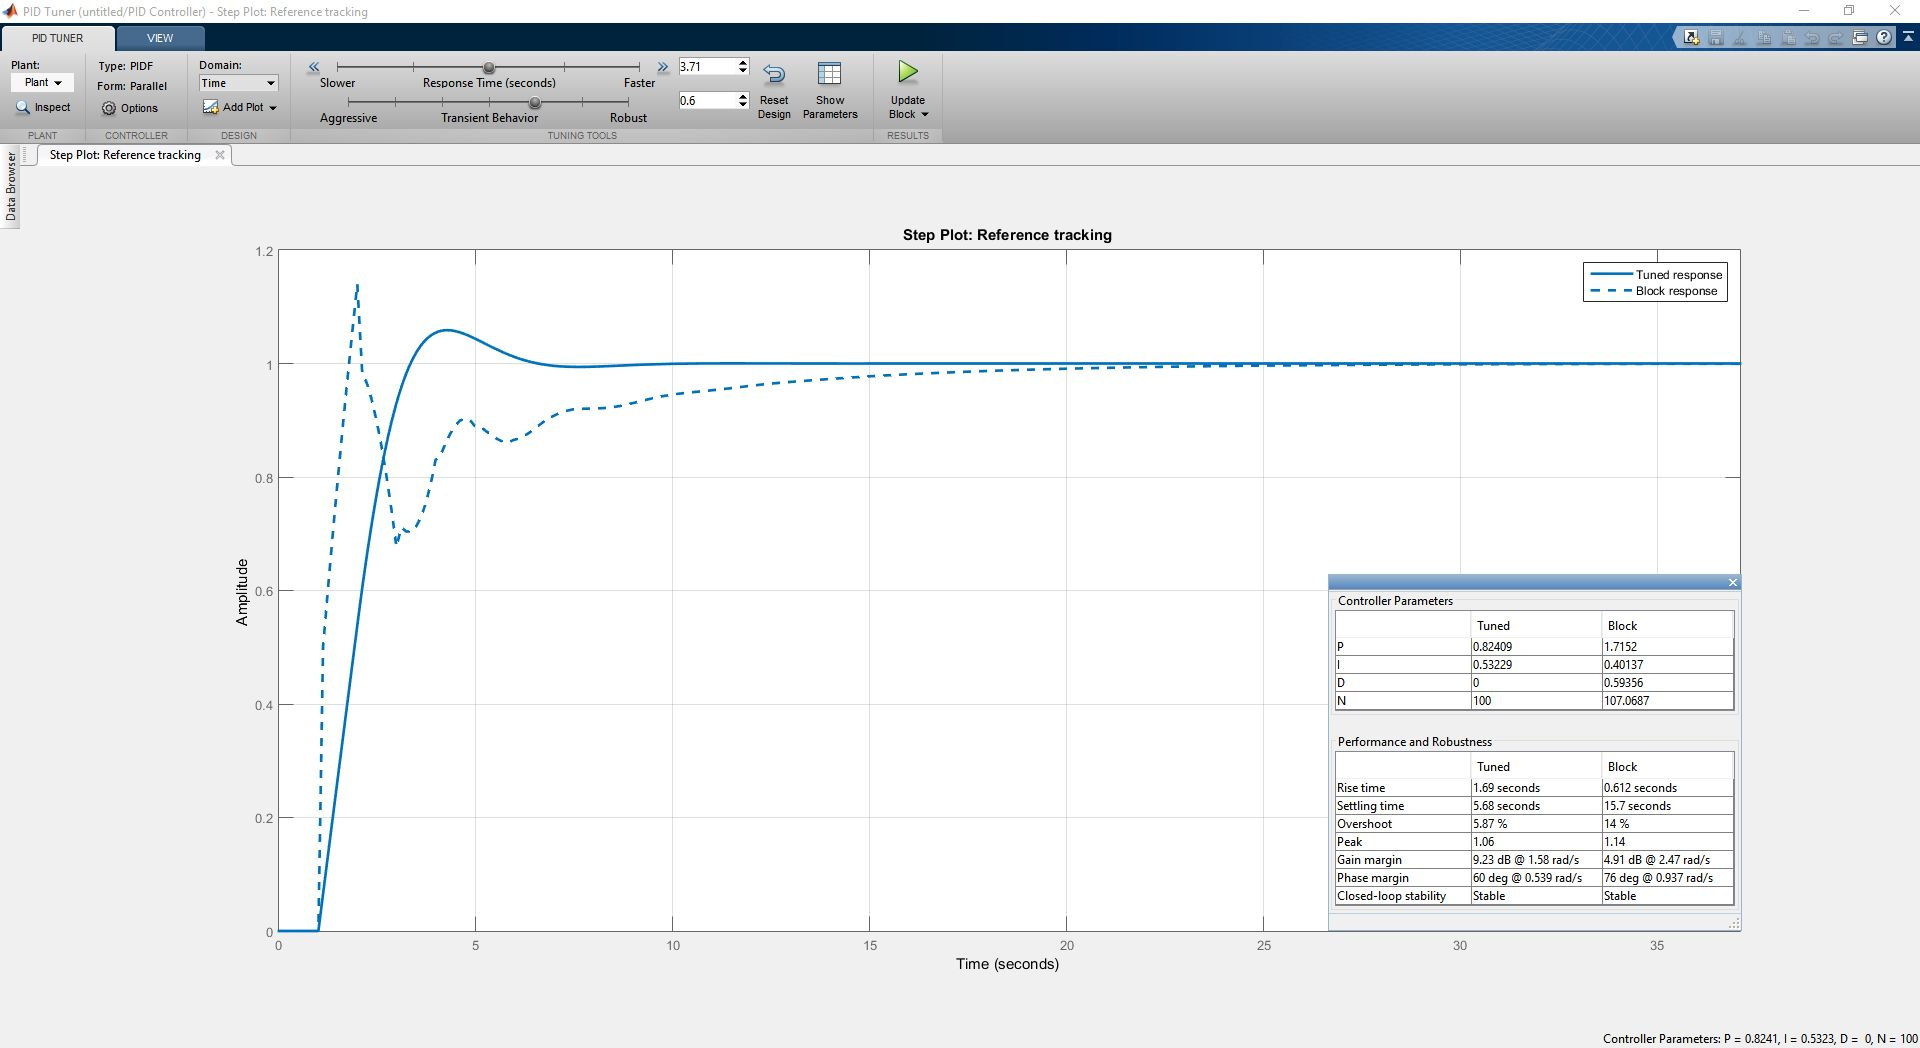
\includegraphics[width=160mm]{PID_Tuner}
	\caption{Zrzut ekranu przedstawiający narzędzie PID Tuner}
	\label{fig:PID_Tuner}
\end{figure}

\noindent Otwiera się wówczas okno, które bazując na podanym modelu wyświetla jego aktualną odpowiedź. Użytkownik jest w stanie zmienić typ regulatora, domyślnie pozostając przy PID. Korzystając z suwaków, można modyfikować czas reakcji oraz agresywność odpowiedzi. Podczas takich zmian, użytkownik na bieżąco obserwuje odpowiedź układu oraz zmieniające się parametry regulatora.
Możliwe jest również wyświetlenie innych przebiegów - takich, jak odpowiedź układu otwartego, odpowiedź skokowa obiektu regulacji - w dziedzinie czasowej lub częstotliwościowej.




\section{SISO Design Tool}
\label{sec:wpr_pidtune}
Kolejne narzędzie do tworzenia regulatorów i filtrów wejściowych dla
układów o jednym wejściu i jednym wyjściu. Program posiada wygodny interfejs umożliwiający bieżący podgląd charakterystyk czasowych i częstotliwościowych
zarówno układu otwartego (dla regulatora) oraz zamkniętego (obiekt + regulator). Użytkownik definiuje układ poprzez wybór jednego ze schematów, podaje wartości obiektów (np. z Workspace'a), a następnie przechodzi do zakładki poświęconej strojeniu.
Narzędzie uruchamia się poprzez wpisanie komendy

\textit{controlSystemDesigner}.

\begin{figure}[H]
	\centering
	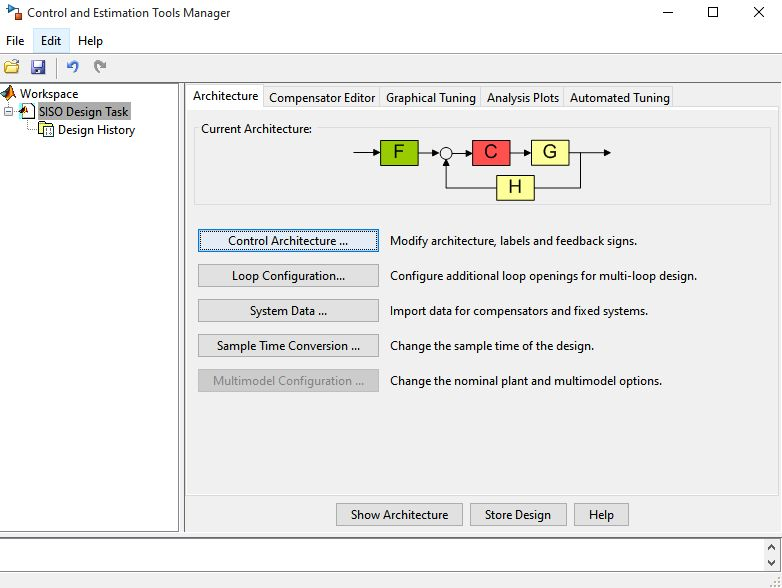
\includegraphics[width=130mm]{SISO_Design_Tool1}
	\caption{Zrzut ekranu przedstawiający narzędzie definiowanie obiektu w SISO Design Tool}
	\label{fig:SISO_Design_Tool1}
\end{figure}
\begin{figure}[H]
	\centering
	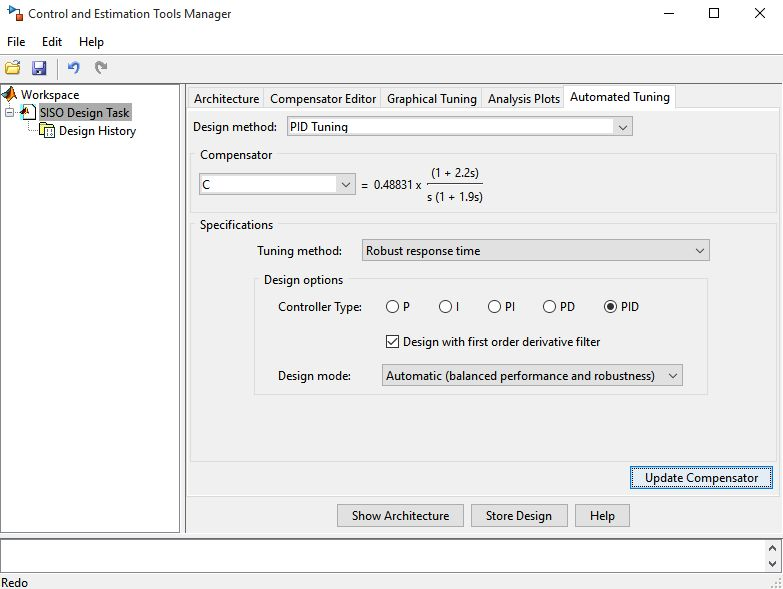
\includegraphics[width=130mm]{SISO_Design_Tool2}
	\caption{Zrzut ekranu przedstawiający proces automatycznego strojenia w SISO Design Tool}
	\label{fig:SISO_Design_Tool2}
\end{figure}





\section{Strojenie z wiersza poleceń}
\label{sec:wpr_Command_Line_Tuning}
Ostatnim i zarazem wykorzystanym w niniejszym projekcie sposobem jest strojenie regulatora za pomocą komendy uruchamianej w skrypcie. Umożliwiło to automatyzację działań. Polecenie

\textit{pidTune(sys,type,opts)}.

\noindent zaprojektuje regulator typu \textit{type} dla obiektu \textit{sys} w pętli sprzężenia zwrotnego. Funkcja zwraca  obiekt \textit{pid} oraz informacje na temat:
\begin{itemize}
	\item Stabilności,
	\item Częstotliwości crossover,
	\item Zapas fazy.
\end{itemize}
Komenda pozwala dodać opcje modyfikujące  domyślne ustawienia strojenia. Są to:
\begin{itemize}
	\item Zapas fazy (domyślnie 60),
	\item Tryb strojenia (domyślnie \textit{balanced}),
	\item Ilość niestabilnych pierwiastków.
\end{itemize}